\documentclass[10pt,letterpaper]{article}
\usepackage[margin=0.76in,headheight=16pt]{geometry}
\usepackage[T1]{fontenc}
\usepackage[utf8]{inputenc}
\usepackage{lmodern,microtype,graphicx,booktabs,tabularx,array,longtable,enumitem}
\usepackage[table]{xcolor}
\usepackage{amsmath,fancyhdr,titlesec,tcolorbox,listings}
\usepackage{xurl,hyperref}
\definecolor{ink}{HTML}{16354A}
\definecolor{teal}{HTML}{127B88}
\definecolor{pale}{HTML}{EDF5F8}
\definecolor{muted}{HTML}{516776}
\hypersetup{colorlinks=true,linkcolor=teal,urlcolor=teal,pdftitle={Steam Patch Intelligence: Architecture and Delivery Plan},pdfauthor={Architecture design for ENSF 621}}
\pagestyle{fancy}\fancyhf{}
\fancyhead[L]{\small\color{muted}STEAM PATCH INTELLIGENCE}
\fancyhead[R]{\small\color{muted}Architecture v1.0}
\fancyfoot[L]{\small\color{muted}Design proposal \textbullet\ 16 October 2026}
\fancyfoot[R]{\small\thepage}
\titleformat{\section}{\Large\bfseries\color{ink}}{\thesection}{0.7em}{}
\titleformat{\subsection}{\normalsize\bfseries\color{teal}}{}{0em}{}
\setlength{\parindent}{0pt}\setlength{\parskip}{6pt}
\setcounter{tocdepth}{1}
\setlist[itemize]{leftmargin=1.4em,itemsep=3pt,topsep=4pt}
\setlist[enumerate]{leftmargin=1.6em,itemsep=3pt,topsep=4pt}
\renewcommand{\arraystretch}{1.2}
\newcolumntype{Y}{>{\raggedright\arraybackslash}X}
\newcommand{\sr}[1]{\hyperlink{src#1}{\textcolor{teal}{[#1]}}}
\newcommand{\key}[1]{\textbf{\color{ink}#1}}
\newcommand{\nextsection}[1]{\clearpage\section{#1}}
\newenvironment{decision}{\begin{tcolorbox}[colback=pale,colframe=teal,boxrule=0.5pt,arc=2pt,left=9pt,right=9pt,top=6pt,bottom=6pt]}{\end{tcolorbox}}
\lstset{basicstyle=\ttfamily\footnotesize,breaklines=true,columns=fullflexible,keepspaces=true,frame=single,rulecolor=\color{pale},backgroundcolor=\color{pale},aboveskip=7pt,belowskip=7pt}
\begin{document}
\begin{titlepage}
\vspace*{0.7in}
{\color{teal}\large ENSF 621 \quad / \quad SYSTEM DESIGN}\par
\vspace{0.3in}
{\fontsize{35}{40}\selectfont\bfseries\color{ink}Steam Patch\\Intelligence}\par
\vspace{0.25in}
{\Large Architecture, model strategy, data evaluation,\\and a phased path to production}\par
\vspace{0.5in}
\begin{decision}
\large Turn Steam reviews and developer announcements into patch reports that explain which changes players like, which they dislike, and what the available evidence supports.
\end{decision}
\vspace{0.35in}
\key{Prepared for}\par
Faiz Marsad and Ahmad Faisal Mirza\par
ENSF 621 project repository\par
\vspace{0.2in}
\key{Design baseline}\par
Repository data and proposal inspected on 16 October 2026.\par
Official API and tooling documentation checked during preparation.\par
Version 1.0 \quad | \quad Architecture proposal; no new model results claimed.\par
\vfill
{\color{muted}Includes the local MVP, reliability and evaluation work, production MLOps, decision rationales, acceptance gates, and implementation priorities. The accompanying source and diagrams are editable.}
\end{titlepage}

\section*{Executive recommendation}
\addcontentsline{toc}{section}{Executive recommendation}
Build a \key{modular Python application with a separate durable worker}, rather than starting with independently deployed microservices. Use FastAPI for contracts, Streamlit for the first interface, PostgreSQL with pgvector for application data, and immutable Parquet snapshots for offline analysis. Most analysis runs in background jobs; the interface reads versioned report snapshots.

Keep the proposed three phases, but change what they mean:
\begin{enumerate}
\item \key{Phase 1: a trustworthy end-to-end MVP.} Search for a game, fetch data on demand, select a patch, and show cited change-level feedback. Include essential tests, schemas, dataset identity, and basic experiment logs immediately.
\item \key{Phase 2: measured quality and operational reliability.} Create human labels, evaluate attribution and polarity separately, improve models only where errors justify them, add recovery and load testing, and formalize DVC and MLflow workflows.
\item \key{Phase 3: repeatable production delivery.} Deploy the same application with managed storage, CI/CD, immutable release manifests, controlled model promotion, monitoring, backups, and rehearsed rollback.
\end{enumerate}

\key{The model recommendation is a small pipeline, not one universal model.} Start with BM25 plus \texttt{all-MiniLM-L6-v2} retrieval. Use the observed Steam recommendation for recommendation trends. Trial a pretrained three-class sentiment classifier for unambiguous review spans, explicitly marked provisional. Train change-targeted polarity and fix-status classifiers only after collecting task-specific labels; compare TF--IDF/logistic regression against DistilBERT before choosing a production champion.

\key{Preserve the proposal's contribution.} The document \emph{Fixed or Only Promised?} defines evidence-backed fix-status checking. This becomes a companion capability, sharing the parser, retrieval, evidence store, and evaluation infrastructure with the broader patch-feedback product. A developer announcing a fix and players reporting improvement remain separate observations.

\begin{decision}
\key{Three product rules govern the architecture.} Every conclusion links to evidence. Every percentage identifies its denominator and collection window. The system can return ``insufficient evidence'' when coverage or model confidence is inadequate.
\end{decision}

\key{Practical scope.} Deliver a local, reproducible course system by 4 December 2026; treat public hosting and production operations as a subsequent release. The live system can accept arbitrary public Steam app IDs, but language, API access, patch-note availability, and review volume determine how much analysis is possible. ``Real time'' means live lookup and bounded refresh, with freshness shown to users.

\clearpage
\begingroup
\setlength{\parskip}{0pt}
\small\tableofcontents
\endgroup

\nextsection{Product scope and meaning of an answer}
The primary user is a community manager, developer, or player investigating a particular update. The core journey is: search a game, select a patch or date window, inspect an overview, drill into individual changes, and open the supporting patch passages and review excerpts.

\begin{tabularx}{\linewidth}{p{1.25in}YY}
\toprule
Capability & Output & Evidence requirement \\
\midrule
Game overview & Recommendation trend, review volume, common themes & Query policy, time range, sample size, freshness \\
Patch reception & Feedback observed around an update & Verified or qualified patch time; complete/partial window \\
Change feedback & Positive, negative, mixed, or unclear feedback per change & Review spans linked to that particular change \\
Fix-status checker & Acknowledged, planned, workaround/partial, limited fix, released fix & Announcement passage plus title, headings, branch and platform \\
\bottomrule
\end{tabularx}

\subsection{What ``went right'' and ``went wrong'' mean}
These are interface summaries of observed feedback. A positive game recommendation does not mean every patch change was liked. A negative review can praise a new map while criticizing weapon balance. Store and classify each relevant review span against the specific change; then aggregate distinct review IDs for that change.

The interface should say ``players discussing this change praised faster loading'' rather than assert that the patch improved everyone's experience. A before/after recommendation difference is descriptive. Sales, outages, review campaigns, and simultaneous hotfixes can change the same numbers. Causal impact estimation is a separate research project.

\subsection{Scope assumptions and explicit extensions}
The MVP is English-only, CPU-first, and intended for the existing two-person team. It processes public reviews and developer announcements; it does not verify installed builds or run the game to test fixes. Use the existing 30 games for development and research, while allowing new app IDs through the live connector.

The latest request expands the proposal's original local-only, 30-game scope. Preserve its five-level ladder and four-system comparison as the research track. Add patch sentiment as a product track with its own labels and evaluation. Hosted production, multilingual models, external publisher websites, account subscriptions, and optional generated narratives are later extensions with separate acceptance criteria.

\subsection{User-visible states}
Display \texttt{queued}, \texttt{collecting}, \texttt{analyzing}, \texttt{ready}, \texttt{partial}, or \texttt{failed}, plus progress and last successful refresh. Distinguish ``no patch notes found,'' ``not enough reviews,'' ``unsupported language,'' and ``source temporarily unavailable.'' These states explain missing results without turning absence of evidence into a negative conclusion.

\nextsection{What the repository actually contains}
The evidence file \texttt{evidence/repository\_audit.json} records CSV row counts, columns, timestamps, uniqueness checks, and SHA-256 fingerprints. Counts below were recomputed from the actual CSVs rather than copied only from the proposal.

\begin{tabularx}{\linewidth}{Yrr}
\toprule
Dataset / property & Observed count & Interpretation \\
\midrule
English reviews & 73,336 & 30 games \\
Negative recommendations & 13,895 & 18.95\% of collected reviews \\
Reviews with fewer than 10 words & 42,548 & 58.02\%; retain for trends \\
Reviews with at least 10 words & 30,788 & Candidate detailed-text pool \\
Balanced text export & 30,000 & Exactly 1,000 per game \\
Negative in balanced text export & 7,517 & 25.06\%; different population \\
Edited reviews in full export & 3,470 & 4.73\%; no original edit history \\
Developer announcements & 3,445 & Includes marketing and other news \\
Rule-flagged patch candidates & 890 & Screening results, not patch labels \\
Posts marked manually verified & 10 & Existing metadata, not independently relabelled here \\
\bottomrule
\end{tabularx}

Review creation dates span 14 January--14 October 2026 (UTC). There are 56,840 reviews created in September or October: 77.51\% of the full collection. Announcement dates span 9 October 2024--14 October 2026. Per-game announcement counts range from 1 to 300; the upper cap is not evidence of complete history.

\key{Existing strengths.} The collector supports the modern review service, cursor checkpointing, persisted HTTP cooldowns, privacy filtering, write recovery, and duplicate detection. The exports include recommendation, creation/update times, review text, playtime, game ID, keyword flags, and source links. There are already 15 tests.

\key{Observed readiness gaps.} Running \texttt{python -m unittest discover -s tests -v} from the project root produced 10 passes and 5 errors. The default snapshot is \texttt{raw/steam\_30\_games}, but argument validation rejects slashes. Five recovery tests hit this invalid default. Record this as the first implementation fix; this architecture task does not modify it. The full output is in \texttt{evidence/existing\_tests.txt}.

The checkout contains snapshot manifests but not the per-game raw payload folders. The CSV announcement export has cleaned text, not a faithful heading tree. Proposal references to older output paths and some audit scripts do not match the present checkout. Its historical ``15 passing tests'' statement therefore cannot be treated as current verification. Also, \texttt{analysis.json.total\_short} means at most five words, whereas the ten-word subset excludes 42,548 rows: these are different definitions.

\nextsection{Data inspection before model selection}
\begin{decision}
\key{First decision: separate data suitable for counting from data suitable for text modelling.} Use all eligible collected reviews for recommendation statistics. Use an explicitly labelled text subset for detailed analysis. Never present the per-game capped export as the overall public recommendation distribution.
\end{decision}

\begin{tabularx}{\linewidth}{p{1.0in}YY}
\toprule
Inspection & Checks and artifact & What the finding changes \\
\midrule
Integrity & CSV BOM handling; types; IDs; duplicates; timestamp order; hashes; missing fields & Invalid rows are quarantined; schema failures block publication \\
Coverage & Per-game/day counts; API caps; earliest/latest times; exhausted pages; requested/observed ranges & Incomplete patch windows trigger backfill or a partial report \\
Sampling & Recommendation rate by game, length, purchase policy and time & Keep counting population separate; report sensitivity analyses \\
Source quality & News vs patch; HTML/BBCode; heading preservation; branch/platform; external links & Recover original formatting; add parser fixtures and review ambiguous posts \\
Text quality & Language mismatch; empty/meme text; duplicates; negation; sentence boundaries; slang & Retain short signals; route unsupported or ambiguous spans to abstention \\
Label quality & Class counts; agreement; difficult negatives; rare platforms and status levels & Revise guide; collect missing labels before adding model complexity \\
\bottomrule
\end{tabularx}

\subsection{Concrete analysis outputs}
Produce a versioned profiling report with per-game calendar heatmaps, missing-value tables, review-length histograms, recommendation distributions, duplicate clusters, edit rates, and patch coverage matrices. Include examples of errors in the parser, not only aggregate scores. Avoid using live, changeable API results as the reproducibility input.

Cross-check computed counts against saved summaries, investigate discrepancies, and document the exact meaning of every field. Import CSVs using \texttt{utf-8-sig}; otherwise the first column is a BOM-prefixed app ID. Keep source timestamps in UTC and convert them only at presentation time. Do not reuse the overlap-analysis stop-word list for polarity or status: it removes ``not'' and ``no'', which can reverse the meaning of a fix claim.

\subsection{Model selection follows error analysis}
Start with an inspected sample of approximately 100 patch claims and 200 review spans spread across games, dates, lengths and recommendation labels. This is a feasibility sample, not a final test set. If relevant passages are absent from top candidates, improve retrieval and parsing. If candidates are present but wrong entities link, improve relevance. If links are correct but sentiment is wrong, collect polarity labels. If title or heading changes flip the meaning, prioritize context-aware status classification. A larger language model does not repair missing source coverage.

\nextsection{High-level architecture and boundaries}
\begin{center}
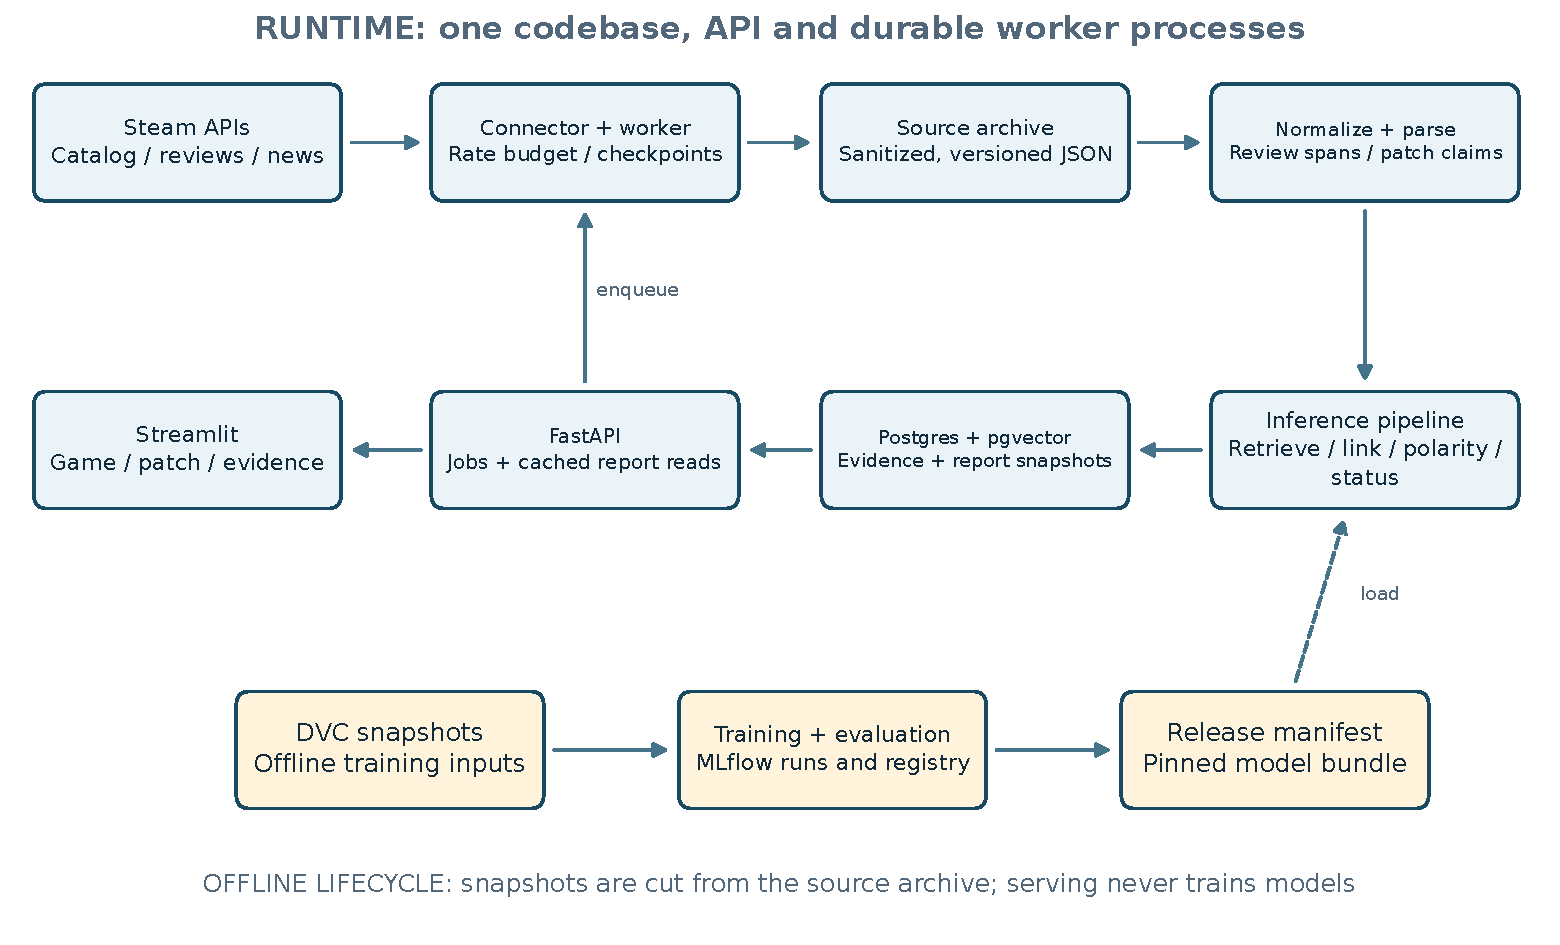
\includegraphics[width=\linewidth]{figures/system.pdf}
\end{center}
\vspace{-4pt}
\key{Runtime path.} Steam connectors write sanitized source records before derived processing. The worker validates and parses those records, computes predictions, and atomically publishes an analysis snapshot. The API reads published results and enqueues refreshes. The interface does not perform collection or run training in a page request.

\key{One repository; separate processes.} Organize ingestion, parsing, retrieval, inference, aggregation, and serving as modules behind typed interfaces. The API, worker, and training commands import the same transformation and inference code. Deploy them separately only to isolate latency, resource usage, and failures. This avoids early distributed-service overhead while leaving clear extraction points later.

\key{Storage roles.} PostgreSQL owns game metadata, jobs, normalized entities, evidence links, and report pointers. pgvector stores embeddings alongside relational keys and supports exact or approximate search.\sr{12} Parquet snapshots support repeatable offline analytics with DuckDB. The source archive is a local directory in Phase 1 and private object storage in production.

\key{Training and serving boundary.} DVC identifies approved offline snapshots. MLflow records training/evaluation and model artifacts. Runtime loads a pinned inference bundle; neither the UI nor a game lookup can trigger model promotion. The service continues using its last verified bundle if the tracking server is unavailable.

\nextsection{Steam API integration and realistic freshness}
Official Valve documentation has changed since many older tutorials. Use adapters with explicit endpoint versions and contract tests; keep legacy support only for replaying an existing saved cursor.

\begin{tabularx}{\linewidth}{p{1.1in}YY}
\toprule
Purpose & Preferred integration & Rationale / limitation \\
\midrule
Game catalog & \texttt{IStoreService/GetAppList/v1} & Key required; paginate with last app ID and use modified-since sync. Search the cached catalog locally.\sr{2} \\
Reviews & \texttt{IUserReviewsService/GetAppReviews/v1} & Current replacement for deprecated store appreviews; typed filters and JSON service input.\sr{1} \\
Announcements & \texttt{ISteamNews/GetNewsForApp/v2} & Request full content and developer feed; paginate by publication cutoff. News still requires patch classification.\sr{3} \\
Build history & No general public build lookup dependency & Build and beta methods require an owning publisher key. Do not assume access for arbitrary games.\sr{4} \\
\bottomrule
\end{tabularx}

\subsection{Review adapter contract}
Send \texttt{input\_json}; Recent=1, Updated=2, all review types=0, all purchase types=1. Page size is at most 100. Include off-topic periods explicitly with \texttt{filter\_offtopic\_activity=false}. Date filtering requires both start and end. Inspect HTTP status; the modern response has no legacy success flag. Anonymous responses may be cached for ten minutes and have a shared lower rate limit.\sr{1}

Use Recent for new reviews and Updated for edit reconciliation. Store query policy with each collection, and recheck adapter fixtures before deployment. This endpoint contract is distinct from the application's model or report schema.

\subsection{Lookup and source constraints}
Do not rely on the deprecated \texttt{ISteamApps/GetAppList/v2}.\sr{4} A catalog sync supports name/typeahead lookup without a network call per keystroke. At selection, enqueue a live refresh. Accept a numeric app ID or canonical Steam app URL when catalog credentials are absent; the UI then states that name search is unavailable until configured.

For news, request \texttt{maxlength=0} and \texttt{feeds=steam\_community\_announcements}.\sr{3} Preserve original formatting before cleaning. A post can point to a publisher website or omit the full patch; return partial coverage and a link. External crawling is a later allowlisted adapter, not an implicit arbitrary URL fetch.

\begin{decision}
\key{Freshness promise.} Live requests refresh available source data, not an instantaneous worldwide stream. Target hourly active-game polling and on-demand refresh, always showing collection time and analysis time. Steam's upstream caching and throttling can dominate freshness. No assumption of a guaranteed webhook or complete patch history is required.
\end{decision}

\nextsection{Ingestion, incremental refresh, and recovery}
\subsection{A new game request}
The API validates the app ID, creates or reuses a job, returns HTTP 202 with a job URL, and immediately serves any existing report. A worker first fetches metadata, recent reviews, and announcements. It then backfills only the selected patch window or configured history budget. Fresh data is useful before full history is complete; the report carries a coverage state.

\key{Phase 1 job mechanism.} Use a PostgreSQL jobs table and a polling worker. Claim a job transactionally using row locks with \texttt{SKIP LOCKED}; record a lease owner, heartbeat, deadline and attempts. A partial unique index prevents duplicate active jobs for the same game, policy and operation. Start with one worker. This provides durable progress without adding a broker immediately.

\subsection{Incremental algorithm}
\begin{enumerate}
\item Keep independent backfill cursors and forward-refresh checkpoints per app, endpoint, mode, and query policy. A completed snapshot is frozen; it is not a live refresh.
\item Start forward scans at the newest page, with a bounded overlap such as 48 hours. Recent mode discovers new records; Updated mode detects changed old reviews. Use source update timestamps as the edit watermark, with an overlap and a periodic deeper reconciliation.
\item Write a sanitized, checksummed source batch durably. Upsert reviews by app ID and review ID. Append a new revision only when tracked fields change; deduplicate the source page and revision content independently.
\item Advance the cursor only after durable persistence. Job retries may repeat requests; database constraints and deterministic derived keys make repeated processing safe.
\item Recompute only affected windows and report generations. Publish the new generation atomically after validation. Retain the previous report on failure, visibly marked stale.
\end{enumerate}

\subsection{Rate budgets and failure handling}
Retain the collector's three-second spacing as an initial operational setting, not a guaranteed safe rate. Valve's published Web API terms state a 100,000-call daily ceiling; lower endpoint throttles still apply.\sr{5} Coordinate a global request budget across workers, honor Retry-After, add jitter, and prioritize interactive refreshes over backfill. More worker replicas must not multiply upstream request allowance.

Timeouts and transient 5xx errors receive bounded retries. Repeated 429s defer the durable job rather than sleeping a worker indefinitely; persist the cooldown so restart cannot bypass it. Authentication failures and schema changes fail clearly and alert the maintainer. Review and news jobs can succeed independently, producing a partial report when one source is unavailable.

News pagination needs explicit boundary tests: same-second posts, duplicates, unchanged pages, and source caps. Preserve all returned IDs before moving the cutoff; label completeness unknown when the interface cannot prove all items were retrieved. Periodic rescan is needed for edited announcements and missing/deleted sources, which the feed may not signal directly.

\nextsection{Data model, contracts, and lineage}
\begin{tabularx}{\linewidth}{p{1.28in}YY}
\toprule
Entity & Key and essential fields & Why it exists \\
\midrule
Game & App ID; display name; catalog version; last sync & Stable identity independent of game title \\
Collection batch & Batch ID; endpoint; policy; cursor; timestamps; raw URI; checksum; coverage & Reproduce what was actually available \\
Review revision & App ID + review ID + revision hash; created, updated, observed times; recommendation; text; author pseudonym & Preserve edits without rewriting historical analyses \\
Announcement revision & App ID + news ID + content hash; title; original markup; published/observed times; URL & Detect post edits and preserve document context \\
Patch / claim & Patch ID; source revision; heading path; exact offsets; action/entity; release time; platform/branch; verification & Separate news, release events, and individual changes \\
Review span & Review revision + offsets; exact quote; normalized text & Attribute sentiment to a span, not the whole review \\
Evidence link & Claim + span + inference bundle; relevance, polarity, status, abstention reason & Trace each conclusion back to both sources \\
Analysis snapshot & Game/patch/policy/window; coverage; input hashes; bundle; aggregates; published time & Serve reproducible reports and safe rollback \\
Label / job & Label provenance and adjudication; or lease, retries and state & Separate human truth from predictions; durable work \\
\bottomrule
\end{tabularx}

Use Pydantic for API boundaries, relational constraints for persisted entities, and Pandera or equivalent checks for offline tables. Validate required fields, positive IDs, UTC timestamps, valid enum values, unique keys, finite vectors of the expected dimension, and resolvable evidence offsets. Preserve unknown optional fields in the source archive; quarantine invalid essential fields.

\key{Time semantics.} Store event time (review creation or claimed release), source update time, and observation time separately. News publication time is a proxy for release time unless the post states a different release. Record the time source and confidence. Never infer that a player installed the latest build from review time alone.

\key{Identity semantics.} A parser version and source revision are part of a claim's derived identity. Fixing the parser can change boundaries, so label migrations require review. Preserve human labels against the exact original revision and offsets. New embeddings get an encoder revision namespace; never compare vectors from different encoders as if they share one space.

\nextsection{Temporal attribution and honest aggregation}
\subsection{Two directions of time}
\key{Patch reception:} start from a released change and retrieve review spans created after that release, normally in a seven-day window. Use a seven-day pre-window for a descriptive baseline. If another update lands sooner, truncate the isolated window or label it as overlapping; do not silently assign all later reviews to both patches.

\key{Fix-status checking:} start from a complaint and retrieve relevant announcement claims. Allow a later announcement only for an explicitly selected ``addressed by now'' question. In historical ``as of'' mode, filter every source and revision by what had been observed by the cutoff. A past patch can also be relevant to a later persistent complaint; its temporal relation must remain visible.

\subsection{Edits and historical reconstruction}
The current snapshot contains latest review text even when the review was edited. For retrospective reception, do not attach text updated after the analysis cutoff to its original creation date. Use a stored revision known at that time, or exclude the edited record from the historical text analysis and disclose the exclusion. Matching creation and update timestamps is only an available proxy for no recorded edit; it is not a full historical guarantee.

The current recommendation field is also a snapshot value. It cannot reconstruct a historical daily recommendation rate before an edit unless earlier revisions were saved. Show current-state-by-creation-date charts distinctly from true point-in-time charts. Continue collecting revisions so this limitation becomes smaller over time.

\subsection{Statistics with explicit denominators}
For a change $c$, let $N_c^+$ and $N_c^-$ be distinct reviews with confident positive-only and negative-only feedback; let $N_c^m$ be mixed and $N_c^0$ neutral. Resolve conflicting spans within one review to mixed. Report all four counts plus abstentions. If a binary approval share is shown, define it as
\[
 A_c = \frac{N_c^+}{N_c^+ + N_c^-},
\]
and show that binary denominator beside it. Never hide mixed or uncertain feedback. Linked-review coverage is distinct linked reviews divided by eligible reviews in the window; model acceptance coverage is accepted classifications divided by candidate classifications.

Use unweighted review counts by default; helpfulness-weighted summaries are an optional separate view because votes also measure exposure. Deduplicate reviews per change, and disclose that one review can discuss several changes, so change counts do not sum to unique players. Wilson intervals can describe a binary share's sampling uncertainty; they do not account for convenience sampling or model error. Use clustered bootstrap analyses when comparing model or patch estimates across games/reviews.

\key{Reporting policy.} Below 20 linked reviews for a change, show examples and ``limited evidence'' rather than rank it as a clear winner or loser. This is an initial product threshold to tune on development labels, not a statistical guarantee. Mark growing windows provisional, report 3/7/14-day sensitivity when data permits, and keep review campaigns visible rather than assuming negative activity is invalid.

\nextsection{Model strategy: start small and measure each task}
\begin{tabularx}{\linewidth}{p{0.9in}YY}
\toprule
Task & Initial choice & Upgrade condition and rationale \\
\midrule
Patch detection / parsing & Title/body rules plus human verification; retain headings and exact spans & Train a classifier if measured news/patch confusion remains high; formatting recovery comes first \\
Retrieval & BM25 + \texttt{sentence-transformers/all-MiniLM-L6-v2}; reciprocal-rank fusion & Add reranking only when relevance errors persist among retrieved candidates \\
Steam vote trend & Count observed \texttt{recommended} values & No model required; show query population and snapshot semantics \\
Text sentiment MVP & Trial \nolinkurl{cardiffnlp/twitter-roberta-base-sentiment-latest} on single-target spans & Three-class starting point; Twitter domain differs from Steam. It cannot alone establish sentiment toward a named change \\
Targeted polarity & TF--IDF + logistic regression baseline; fine-tune \texttt{distilbert/distilbert-base-uncased} on change/span pairs & Promote the best evaluated model; mixed and ambiguous targets require explicit labels \\
Fix status & Context rules, then TF--IDF/logistic regression and matched DistilBERT variants & Retain proposal A/B/C/D comparison; title, heading and scope are inputs, not stripped metadata \\
Narrative & Deterministic report templates and selected evidence & Optional LLM only after evidence coverage and factuality gates; not required for MVP or production \\
\bottomrule
\end{tabularx}

MiniLM produces 384-dimensional embeddings and is intended for sentence/short-paragraph similarity; the model card notes truncation beyond 256 word pieces.\sr{6} Split long material with sentence boundaries and limited context overlap instead of embedding whole patch posts. BM25 preserves rare game entity names that general embeddings may blur. Combine ranks with $\sum_i 1/(60+\mathrm{rank}_i)$, then tune candidate counts on development games; the constant is an initial configuration choice.

The Cardiff checkpoint supplies negative, neutral and positive classes.\sr{7} In Phase 1, accept its polarity only for linked spans with one unambiguous target and no unresolved contradictory clauses; mark other cases mixed/unclear by reviewed rules or abstain. Do not advertise this as validated aspect-based sentiment. Human-labelled target pairs, including hard entity negatives, are required for Phase 2.

DistilBERT is an English base encoder requiring task-specific fine-tuning, not an off-the-shelf fix-status or aspect classifier.\sr{8} Its size makes it a reasonable CPU-serving candidate, but training time and latency must be measured on the team's hardware. Logistic regression is the cheap, inspectable baseline; use word/character features and target--span interactions rather than ignoring the target. Pin checkpoint revisions, tokenizer, preprocessing, thresholds, label map and license metadata. No useful accuracy is assumed before evaluation.

\nextsection{Inference and evidence construction}
\begin{center}
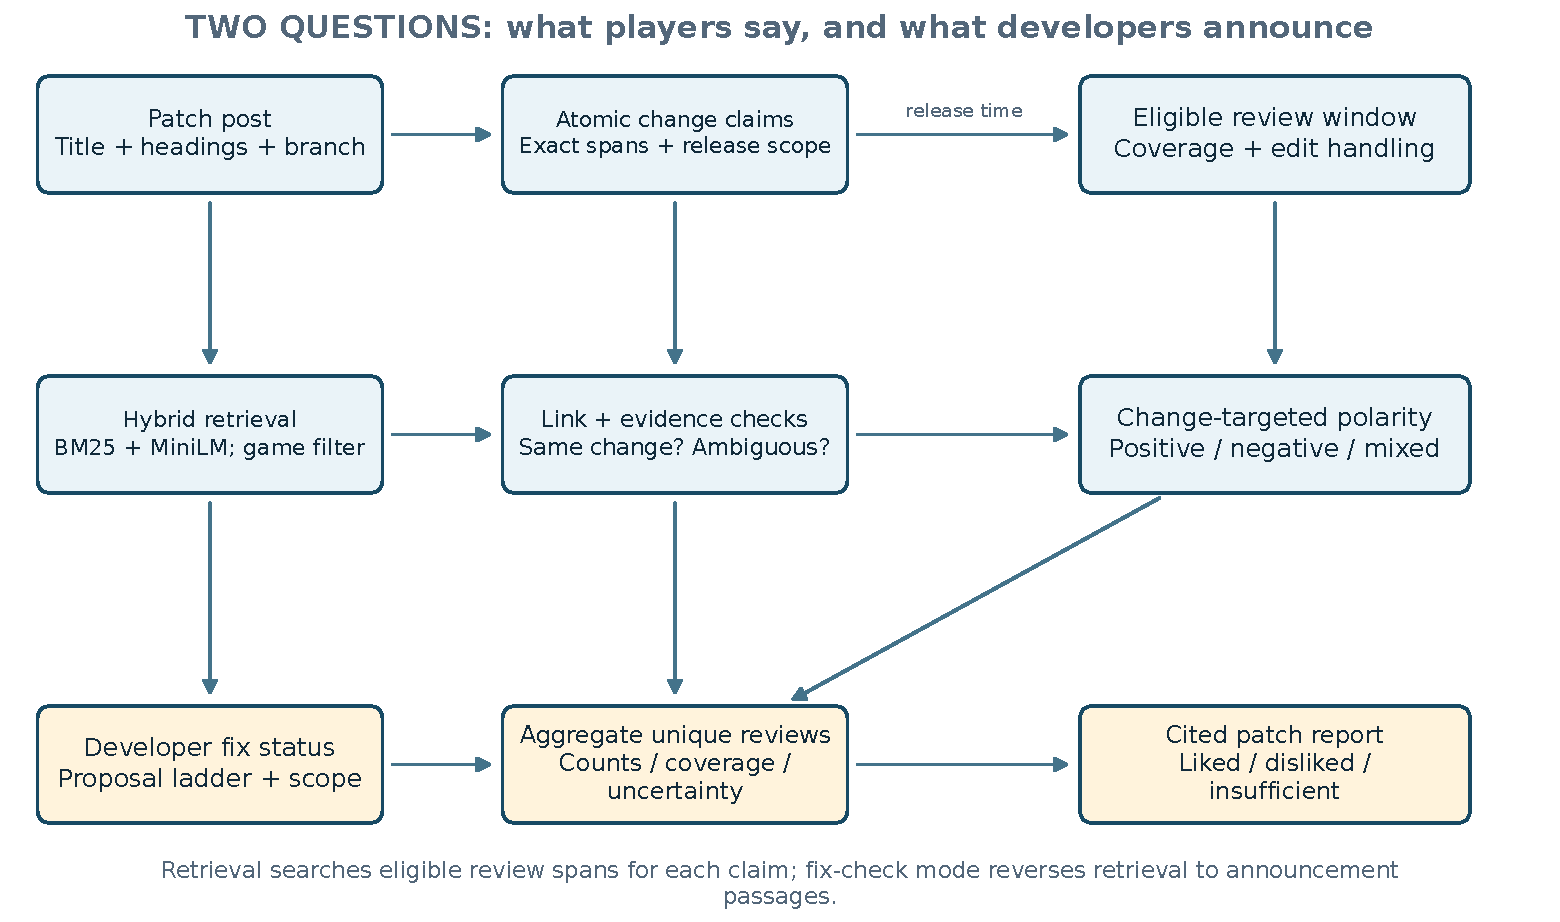
\includegraphics[width=\linewidth]{figures/analysis.pdf}
\end{center}

\subsection{One concrete example, entirely illustrative}
A patch says ``Reduced reload time for the Scout rifle'' under a released balance section. A review says ``Love the faster reload, but the new matchmaking is awful.'' Extract two targets. Link the reload span to the Scout change only if the rifle identity is supported; score it positive. Keep the matchmaking complaint as a separate theme unless a matching change exists. If the entity is ambiguous, show the excerpt as an unconfirmed candidate and exclude it from confident change counts.

\subsection{Retrieval, relevance, polarity and status are separate decisions}
Retrieve the top 20 lexical and top 20 vector candidates within the same game and eligible temporal partition, fuse, and retain the top 10. These are starting budgets, tuned on development data. For a low-volume game exact cosine search is simpler than an approximate index. Use pgvector HNSW only after benchmarks justify it and verify recall under game/time filters.\sr{12}

A relevance threshold or trained pair classifier accepts ``same change/problem'' independently of polarity. An optional \texttt{cross-encoder/ms-marco-MiniLM-L6-v2} reranks only the small candidate set; its score is not a calibrated match probability. Cross-encoders jointly score pairs, whereas bi-encoders permit reusable document embeddings.\sr{9}

The status classifier reads the complaint, passage, heading path, title, neighboring lines and explicit branch/platform. Keep the proposal's five display levels, but model status categorically and store scope independently: limited fixes and workarounds are not universal numerical progress steps. Resolve multiple scopes into separate claims. Source quotes must be exact substrings with validated offsets; attention weights or invented explanations do not count as evidence.

\nextsection{Human labels, evaluation, and promotion gates}
\subsection{Keep the research study and product evaluation distinct}
Preserve the proposal's 500 review/passage pairs (100 pilot and 400 main), approximately 230 development and 270 test labels, and 400 status edits plus 100 originals. These are planned labels, not files found in the current checkout. About 10 development games and 20 held-out games follow the proposal; define inner train/validation partitions within development games. Keep each original, edit family, duplicate cluster, review revision and announcement family within one partition.

Add separate labels for patch identification, review-to-change relevance, target/entity, positive/negative/neutral/mixed polarity, and evidence spans. A course feasibility set of 300--500 target-labelled spans can expose failure modes. A production target of 1,200--2,000 diverse pairs is a planning estimate; learning curves, class coverage and confidence intervals determine whether it is sufficient. Reuse records across tasks only with explicit split alignment and separately defined labels.

Both annotators independently label the pilot before seeing model output. Report agreement for relevance, status and polarity, then adjudicate. Retain the proposal's $\kappa \geq 0.6$ pilot guideline; revise the guide if ambiguity dominates. Include sarcasm, multi-target reviews, short complaints, test branches, promised fixes, incorrect entities and unrelated news. Weak labels from headings are training-only; heuristics never become ground-truth test labels.

\begin{tabularx}{\linewidth}{p{1.0in}YY}
\toprule
Layer & Metric & Initial acceptance policy (proposed, unmeasured) \\
\midrule
Parser & Exact span validity; heading/scope accuracy & 100\% valid stored offsets; report semantic parser errors on gold fixtures \\
Retrieval & Recall@10; nDCG@10 by game & Aim Recall@10 $\geq 0.85$ on adjudicated answerable queries with a pooled relevance set \\
Linking & Precision/recall and risk--coverage & Aim precision $\geq 0.90$ at a declared nontrivial coverage; inspect per-game errors \\
Polarity & Macro-F1; per-class recall; calibration & Aim macro-F1 $\geq 0.75$ and improvement over baseline; no overall accuracy-only gate \\
Fix status & Released-fix precision, recall; all-level confusion; flip accuracy & Aim overclaim rate $\leq 0.10$ with coverage and intervals; meet proposal D-vs-C research rule separately \\
Report & Claim-to-source validity; aggregate consistency & Every displayed numerical assertion recomputes; every qualitative conclusion has valid evidence \\
\bottomrule
\end{tabularx}

\key{Do not manufacture certainty.} Lock thresholds using validation data, then evaluate the held-out test once per declared study. Report 95\% intervals and sample sizes; small data may not certify the target precision. For the proposal's hypothesis, test D's lower overclaim rate against C with a paired, clustered interval and recall loss at most five points. A negative or inconclusive result is valid. New production iterations require fresh evaluation cohorts rather than repeated tuning to that locked test.

\nextsection{Phase 1: trustworthy vertical slice}
\key{Objective:} demonstrate one complete, evidence-backed game-to-patch workflow before investing in sophisticated infrastructure. Start with several games having verified patch posts and usable time windows, then test one previously unseen public app ID.

\subsection{Deliverables and rationale}
\begin{enumerate}
\item \key{Repair the current collection contract.} Resolve the invalid default snapshot, rerun all existing tests, and document the supported run command. Preserve the working retry and recovery logic rather than replacing it wholesale.
\item \key{Import and profile the existing data.} Create typed Parquet snapshots and a PostgreSQL serving schema. Fingerprint CSV inputs; preserve the current data as a named baseline. The profile makes sampling and missing history visible before fitting anything.
\item \key{Implement the shared parser and evidence store.} Reacquire original announcement markup where possible, retaining its new observation date. Do not pretend newly fetched markup is an unchanged historical original. Use a reviewed subset when original context is unavailable.
\item \key{Expose FastAPI and a durable worker.} Add jobs, idempotent persistence, a single global HTTP limiter, and refresh progress. Use Docker Compose for API, worker, UI and PostgreSQL; use a local archive directory initially.
\item \key{Serve a Streamlit dashboard.} Game search/ID input, patch selector, observed recommendation trend, change feedback with provisional polarity, fix-status evidence, and coverage/freshness labels. Use templates rather than generated prose.
\item \key{Include minimum engineering controls.} Lock dependencies, run schema/offset/retry smoke tests in GitHub Actions, track the baseline dataset with DVC metadata, and log baseline experiments in local MLflow. This avoids an untraceable prototype.
\end{enumerate}

\subsection{Exit demonstration}
From a documented local command, ingest a game, restart a worker during a job, resume without duplicated reviews, and open a report with working evidence links. Cached reports must remain readable during a simulated Steam failure. Select a patch with insufficient coverage and verify that the UI explains the limitation. Compare all-review and text-subset recommendation rates to demonstrate that the denominators are deliberate.

\key{Quality gate.} Existing tests pass after the initial fix. New essential boundary tests cover modern response shape, exact evidence offsets, atomic report publication, and one end-to-end fixture. A 100-item human pilot is reviewed. Model outputs remain provisional until measured; no production accuracy claim is required to finish the vertical slice.

\key{Deferred work.} Full retraining automation, multi-region availability, a dedicated vector service, a feature store, Kubernetes, and a narrative LLM provide little value before this slice works. The rationale is team capacity and measured need, not a relaxation of data correctness.

\nextsection{Phase 2: reliability and measured model quality}
\key{Objective:} turn the useful slice into a reproducible and testable product, and complete the research comparison promised in the proposal.

\subsection{Data and model work}
Freeze split manifests and annotation guidelines. Complete the 500 status pairs, the status-flip family, and the separate sentiment feasibility set. Create full-context passages and hard relevance negatives. Train the proposal's passage-only and context-aware variants with matched model families, training data and hyperparameter budgets so context is the intended experimental difference.

For product polarity, first compare the provisional sentence model against a target-conditioned TF--IDF classifier. Fine-tune a target-conditioned DistilBERT model only if labelled class support and learning curves justify it. Use class weighting where appropriate, tune abstention, calibrate confidence on validation data, and report per-game and per-length performance. Avoid random row splits that share game vocabulary, repeated patch wording or edited copies across training and test.

\subsection{Reliability and test expansion}
\begin{tabularx}{\linewidth}{p{1.2in}YY}
\toprule
Test family & Representative cases & Reason \\
\midrule
Unit / property & Negation; ambiguous target; empty text; malformed markup; exact quote slicing; count deduplication & Protect meaning and aggregation invariants \\
Adapter contract & Recorded modern API payloads; missing optional fields; 429/Retry-After; endpoint migration & Catch upstream/schema changes independently of models \\
Integration & Real Postgres; leases; transaction rollback; source revision change; parser reindex & Validate persistence and recovery semantics \\
Behavioral NLP & ``fixed'' to ``will fix''; known-issue heading; Unstable title; same problem/different entity & Verify sensitivity to evidence and invariance to irrelevant formatting \\
End-to-end & Cold game request; progress; partial results; stale cache; evidence click-through & Protect the actual user journey \\
Performance / failure & Parallel requests; slow Steam; worker kill; lost lease; DB unavailable; oversized notes & Establish resource limits and safe degradation \\
\bottomrule
\end{tabularx}

No network call belongs in ordinary pull-request tests. Use sanitized fixtures and deterministic clocks. A separate scheduled adapter probe can check a low-volume live request and report failures without making unit tests depend on Steam availability.

\key{Exit gate.} DVC can reconstruct an approved offline run; MLflow links metrics to that dataset and code. Publish a model card and a failure-analysis report, including negative results. Report quality metrics with intervals, validate worker recovery and stale-report serving, and establish load-test results for a declared hardware/concurrency budget. A model that fails quality gates stays a candidate; the app retains the simpler verified baseline or abstains.

\nextsection{Phase 3: repeatable production operations}
\key{Objective:} release a validated application and model bundle through an auditable path, and keep it recoverable after deployment. This phase adds infrastructure and operational evidence; it does not by itself make a weak classifier reliable.

\subsection{Production deliverables}
\begin{enumerate}
\item \key{Infrastructure as code.} Provision a chosen cloud environment, private database/object storage, container registry, API/UI/worker services, secrets, scheduler, alerts and backups. Keep development, staging and production state separate.
\item \key{Software CI/CD.} Test a pull request, build and scan an image once, deploy the digest to staging, run migrations and smoke tests, then promote the same digest to production. Protect deployment environments and record the release manifest.
\item \key{Model promotion.} Train on an approved data snapshot, evaluate against defined gates, register a model version, and nominate it for a release. Deploy explicit versions, not a moving ``latest'' model reference.
\item \key{Operational visibility.} Record API latency/errors, source freshness, queue age, ingestion coverage, abstention, label-reviewed quality, and per-game failures. Put the active data/model/report versions in operator diagnostics.
\item \key{Recovery.} Rehearse application rollback, model rollback, source outage handling, database restore, and report rebuild. Backups are successful only when a restore has been exercised.
\end{enumerate}

\subsection{Queue and orchestration decisions}
Keep the PostgreSQL job queue initially in production. It is sufficient for a modest game catalog and avoids a broker migration solely for a diagram. Revisit when measured queue contention, worker scale or isolation needs warrant it. If needed, introduce SQS through the existing job interface, retaining the database as the job/report system of record. A transactional outbox avoids a database/message dual-write gap; consumers remain idempotent.

Continue simple scheduled enqueueing for refreshes. DVC orchestrates reproducible offline dependencies, not a long-running online work queue. Its documentation explicitly distinguishes its lightweight pipeline role from full execution/recovery orchestration.\sr{10} Add Prefect or Airflow only when dependent multi-stage schedules, retries and observability become hard to maintain with the current scheduler.

\key{Exit gate.} A release can be recreated from its manifest; staging matches production interfaces; security and migration checks pass; the quality gate has a recorded decision; a restore and rollback drill meets the provisional recovery objectives. Operations have a named owner. Avoid calling a single untested cloud deployment a full production system.

\nextsection{MLOps: what Git, DVC and MLflow each own}
\begin{tabularx}{\linewidth}{p{0.85in}YY}
\toprule
System & Authoritative contents & Boundary \\
\midrule
Git & Code, tests, contracts, ADRs, configuration, dependency lock, DVC metadata, split manifests & No secrets or growing source archives \\
DVC & Approved raw/normalized training snapshots, labels, offline pipeline dependencies and outputs & Dataset reproducibility; not the live database or hourly archive catalog \\
MLflow & Run parameters, metrics, plots, evaluation artifacts, model signatures and registered versions & Experiment/model lifecycle; not the source of data truth \\
Object store & Sanitized source batches, Parquet objects, DVC remote, MLflow artifacts, release files & Isolate prefixes and permissions; retain checksums and retention policy \\
PostgreSQL & Runtime entities, revisions, jobs, evidence links and published report pointer & Operational state; backup separately from DVC \\
\bottomrule
\end{tabularx}

Git stores DVC metafiles and \texttt{dvc.lock}; the remote stores tracked data objects. A deterministic pipeline can use stages \texttt{validate -> normalize -> parse -> split -> features -> train -> evaluate}.\sr{10} Live collection is a separately authorized snapshot acquisition step, never a hidden network dependency inside an offline training reproduction.

MLflow aliases such as \texttt{candidate} and \texttt{champion} support nomination; deprecated fixed registry stages should not define the workflow.\sr{11} Resolve an approved alias to an immutable model version during release creation. The runtime release manifest pins that version so an alias update cannot silently change a running service.

\subsection{One release identity links every artifact}
\begin{lstlisting}
release: 1.0.0
git_commit: <full commit SHA>
container_digest: sha256:<image digest>
dataset_id: <approved snapshot ID>
dvc_lock_sha256: <hash>
split_manifest_sha256: <hash>
models:
  embedder: {checkpoint: all-MiniLM-L6-v2, revision: <hash>}
  relevance: {registry_name: relevance, version: <integer>}
  polarity: {registry_name: targeted-polarity, version: <integer>}
  fix_status: {registry_name: fix-status, version: <integer>}
pipeline_schema: 1
parser_version: 1
aggregation_policy: patch-window-v1
thresholds_sha256: <hash>
evaluation_artifact: <immutable URI and checksum>
\end{lstlisting}
The specimen is a proposed schema, not an existing release. Package fitted tokenizers, lexical indexes, calibration/threshold configuration and label maps with the model bundle. Training logs record seeds and hardware/library versions; exact bitwise GPU reproducibility is not assumed. Every report records its input revision set and bundle identity, so a data change is distinguishable from a model change.

\nextsection{CI/CD and model release workflow}
\begin{center}
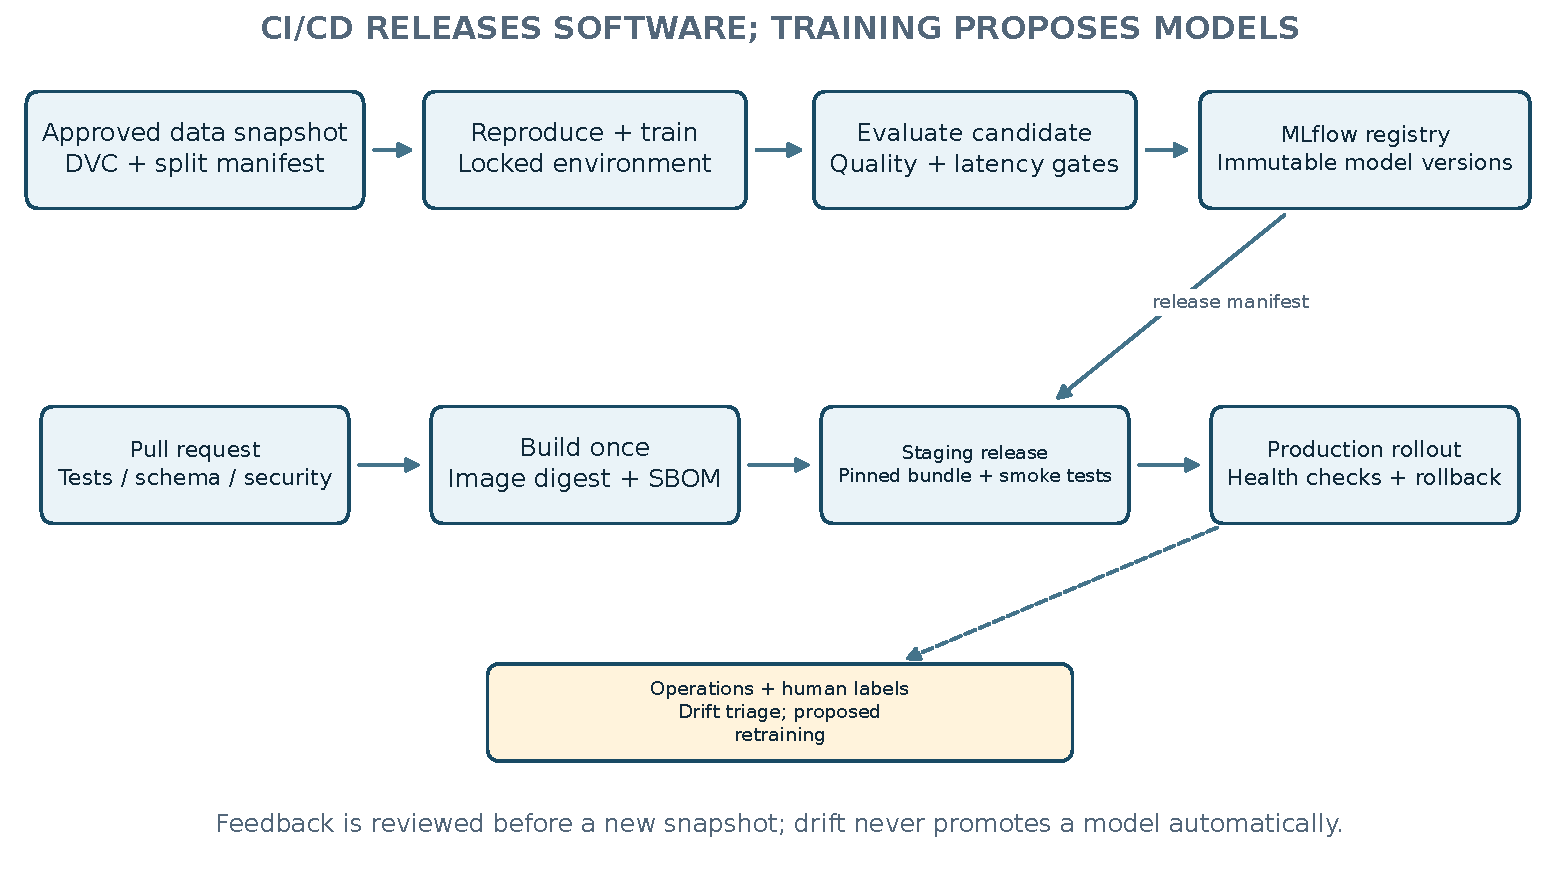
\includegraphics[width=\linewidth]{figures/lifecycle.pdf}
\end{center}

\begin{tabularx}{\linewidth}{p{1.05in}YY}
\toprule
Trigger & Workflow & Gate / artifact \\
\midrule
Pull request & Lint/type checks; unit, schema and integration fixtures; dependency/security checks & No production credentials; reproducible test report \\
Merge / release & Build and scan image; generate SBOM; push by digest; stage deployment & Immutable image and release manifest \\
Approved snapshot & DVC pull/reproduce; train candidates; MLflow logging; evaluation & No automatic champion promotion from a training success \\
Staging passed & Migration compatibility; model load; fixture report; load smoke test & Recorded software/model/data compatibility decision \\
Production promotion & Deploy same image/bundle; monitor health and application metrics & Previous release retained; automatic health rollback plus operator runbook \\
Scheduled operation & Adapter probe; profiling; drift report; backup verification & Issues trigger triage; drift alone does not deploy a new model \\
\bottomrule
\end{tabularx}

Prefer short-lived cloud credentials through GitHub OIDC over long-lived deployment keys. Restrict token trust to the intended repository, branch/environment and role.\sr{13} Pin actions to full commit SHAs, use least-privilege workflow permissions, and treat pull-request content as untrusted input.\sr{14} GPU training, if ever needed, is a separately budgeted job; do not attach sensitive self-hosted runners to untrusted forks.

Use a fast fixture subset for pull requests and the full offline benchmark for candidate releases. Required gates include retrieval/linking/polarity/status metrics, abstention coverage, source-offset validity and report arithmetic. Models are not compared only on aggregate accuracy. Evaluate natural and rare-status challenge samples separately; synthetic flip cases cannot estimate real-world prevalence.

\nextsection{Deployment reference and capacity planning}
\subsection{Recommended production reference: a small AWS deployment}
Use Terraform to provision ECR images, ECS Fargate services for FastAPI/Streamlit/worker, an Application Load Balancer with TLS, RDS PostgreSQL with a supported pgvector extension version, private S3 buckets, Secrets Manager, and CloudWatch. Use separate logical databases and service credentials for application state and MLflow metadata. MLflow stays internal, with artifacts in a restricted S3 prefix. Verify extension availability for the selected RDS engine version.\sr{15}

The API/UI run behind a common hostname; the UI calls API endpoints rather than reading database tables. An OIDC-protected maintainer interface owns labeling, refresh administration and model actions. A public read-only report view is optional; collection-triggering endpoints have quotas and resource budgets. The worker needs outbound Steam access, while the database has no public ingress. Explicitly budget private-network egress, load balancing and database costs; managed services are not automatically free.

\subsection{Rollout, migrations, and availability}
Start with rolling ECS deployments with health checks and a deployment circuit breaker/rollback. ECS supports health-based deployment failure detection.\sr{16} Use schema expand--migrate--contract: new columns are initially compatible with both releases, data backfill is resumable, and removal waits until the rollback window closes. A code rollback cannot undo a destructive database migration.

For a course demonstration, Docker Compose on one machine is adequate, with explicit downtime limits. Production can begin with one service task if downtime is accepted; use at least two API/UI tasks across availability zones and a Multi-AZ database when the availability objective is required. Worker concurrency scales by queue age and CPU only while retaining the global source request budget. Streamlit sessions need suitable routing/session handling and reconnection tests when replicated.

\subsection{Size estimates, not benchmark claims}
One float32 384-dimensional vector occupies 1,536 bytes before row/index overhead. At one vector per 73,336 reviews, the vector payload is about 107 MiB. Four spans per review would be about 430 MiB. Text, revisions, indexes and reports add overhead; measure actual database size after import. The current CSVs total roughly 68 MiB on disk, but they are not a production storage forecast.

At 30 games with three pages of incremental polling per hour, the illustrative load is 2,160 requests/day, before news, catalog, edits, retries and backfill. At the collector's initial three-second spacing, a serialized shared client can start about 1,200 requests/hour; throttling may lower this. Budget backfills explicitly so one popular game cannot consume the interactive queue.

\key{Cost method.} Benchmark 1,000 reviews and 100 patch claims; record CPU-seconds, peak RAM, storage growth and source calls. Estimate monthly cost as compute-hours + database + archive + backup + egress + monitoring + CI/training. Use the chosen region's current calculator at deployment time. This document makes no unverified cloud-price promise and provisions no paid resources.

\nextsection{Monitoring, quality drift, and recovery}
\begin{tabularx}{\linewidth}{p{1.0in}YY}
\toprule
Signal & Measurement & Initial action threshold / response \\
\midrule
API health & Request latency; 5xx; DB pool; ready checks & Alert on sustained $>2\%$ errors or p95 cached-report latency $>2$s for 10 minutes \\
Source freshness & Last successful review/news sync, by game and stream & Flag active-game staleness $>2$h; distinguish upstream outage from worker failure \\
Queue health & Oldest pending age; retries; lease expirations & Investigate interactive queue age $>10$min; defer backfill before adding workers \\
Data quality & Schema failures; duplicate ratio; empty texts; coverage loss & Block invalid report publication; compare to a stable per-game baseline \\
Model behavior & Relevance/polarity mix; abstention; entity and language distributions & Triage change outside baseline; inspect samples before assuming degradation \\
Measured quality & Newly human-labelled precision, recall and evidence errors & Re-evaluate candidate/champion; rollback or reduce coverage if a gate fails \\
\bottomrule
\end{tabularx}

These are proposed operating thresholds, not measured service-level achievements. Set a provisional 99.5\% monthly availability objective for cached report reads, p95 under two seconds at 20 concurrent readers, and an initial cold-job target under five minutes for a bounded 1,000-review ingestion on benchmark hardware. Upstream rate limits can invalidate the cold-job target; show progress rather than blocking the request or hiding the delay.

Input drift is not the same as model-quality drift. A real unpopular patch should change sentiment. Per-game comparisons and human review distinguish topic changes, parser breakage, language changes and actual classifier error. Monitor by review length, unseen game, status class, Steam Deck marker and branch, with minimum cell counts to avoid overinterpreting tiny groups. A false Deck marker is not a reliable desktop-hardware label.

\subsection{Operational runbooks}
\key{Steam unavailable:} preserve the last report, mark it stale, back off and resume the same source job. \key{Bad model:} redeploy the previous pinned inference bundle and rebuild affected report generations; changing the model alone does not remove already published wrong reports. \key{Bad parser/data batch:} quarantine the batch, keep the prior report pointer, and replay from the sanitized source revision after a fix.

\key{Data recovery:} use database point-in-time recovery plus daily snapshots, object versioning, and separately protected manifests. Initial production recovery objectives are RPO at most 24 hours and RTO at most four hours; verify these in a staged restore exercise before promising them. Keep model artifacts available locally to serving tasks so a temporary MLflow outage cannot stop cached reads. Assign one primary maintainer and one backup; course staffing does not justify an unsupported 24/7 promise.

\nextsection{Security, privacy, and data lifecycle}
\subsection{Protect the actual system boundaries}
Keep Steam keys, object-store credentials and author pseudonymization secrets out of Git, DVC metadata, logs and browser code. Some source request URLs include parameters, so store redacted request metadata rather than raw credential-bearing URLs. Use TLS, narrowly scoped service identities, parameterized SQL and restricted database network access. The upstream terms require confidentiality of the Web API key and prohibit implying Valve endorsement.\sr{5}

Render review and announcement text as untrusted content: sanitize markup, escape output, limit lengths and downloads, and disallow script/embedded content. Accept app IDs or canonical Steam URLs; do not let a user supply a fetchable arbitrary URL. Any later external patch-note adapter needs host allowlisting, redirect checks and private-IP blocking. Authorization and request quotas apply to expensive refresh endpoints, not just login pages.

An LLM, if added later, receives source text as data with no tools or authority. It may summarize only structured, cited evidence; validate every returned source identifier and number, and fall back to templates on failure. This limits prompt-injection and hallucination exposure while leaving the core pipeline useful without an LLM service.

\subsection{Pseudonymization is not anonymization}
The existing collector replaces author IDs with salted hashes. Retain that boundary before persistence, or use a versioned keyed HMAC if deliberate cross-snapshot grouping becomes necessary. Restrict the secret; rotating it changes linkage and must be documented. Do not store names, avatars, profile URLs or unneeded hardware attributes. Public review text and review links can still identify a person, so hashes do not make the entire dataset anonymous.

The proposal says to share code, labels and totals rather than review copies, while the present repository includes review CSVs. Resolve the publication policy before making a public release: separate public code/metrics from access-controlled raw text and DVC storage. Do not rewrite Git history or remove existing data as part of this design task. Review reuse rights and attribution requirements for the intended release; technical availability alone is not a dataset redistribution license.

\subsection{Retention and corrections}
Adopt a provisional 90-day active source-text retention policy for the hosted service, with longer curated research snapshots only where justified and access-controlled. Keep aggregate metrics and code longer. A documented correction/removal process must find affected normalized rows, text indexes, vectors, cached evidence, report generations, DVC snapshots and artifact copies; object versioning/backups have their own expiry. Training-data deletion may require model retraining when appropriate. Historical reproducibility is subordinate to applicable deletion requirements: record a tombstone and that an older run can no longer be fully reconstructed.

\nextsection{Architecture decisions and tradeoffs}
Each decision below is a recommendation tied to this repository's scale and team. Revisit it when the stated trigger occurs; none is a claim that one vendor or pattern is universally required.

\begin{tabularx}{\linewidth}{p{0.25in}p{1.18in}YY}
\toprule
ID & Decision & Rationale / rejected alternative & Revisit trigger \\
\midrule
01 & Modular monolith with worker & One codebase minimizes deployment and contract overhead; separate worker protects request latency. Many microservices add coordination before demand exists. & Independent teams, scaling or isolation constraints \\
02 & FastAPI + Streamlit & Typed service contract plus fast Python UI matches current skills; a custom React frontend would delay the model/data work. & Public UX, accessibility or scale exceeds Streamlit limits \\
03 & Postgres + pgvector & Relational provenance, jobs and vectors share transactional keys. Avoid a separate vector database initially. & Measured vector/query bottleneck or dedicated search requirements \\
04 & Parquet + DuckDB offline & Stable portable snapshots and efficient inspection; a warehouse/Spark cluster is unnecessary for current volume. & Data exceeds a single machine or broad analytics concurrency \\
05 & Durable jobs before broker & Database leases support restart and deduplication with one fewer service. In-process background tasks can lose work. & Queue contention or independent consumers justify SQS/outbox \\
06 & Asynchronous refresh, cached reads & Upstream latency/throttles cannot meet interactive guarantees. A request should not wait for a full game backfill. & Always retained; streaming progress can improve UX \\
07 & Hybrid retrieval & Keywords retain exact entity names; embeddings find paraphrases. Either alone has predictable blind spots. & Held-out retrieval analysis favors a simpler or newer encoder \\
08 & Small task-specific models & Different labels and failure costs require separate relevance, polarity and status decisions. One prompted LLM hides error sources and ongoing cost. & Measured end-to-end gain justifies a new evaluated component \\
09 & Exact evidence spans & Quotes, scope and source revisions make conclusions inspectable. Free-text explanations alone are not verification. & Always retained; span extraction may improve \\
10 & Templates first & Predictable counts, citations and failure behavior. Fluent generation is optional polish after quality is established. & User study and factuality tests justify LLM summaries \\
\bottomrule
\end{tabularx}

\nextsection{Decision rationales: quality and operations}
\begin{tabularx}{\linewidth}{p{0.25in}p{1.18in}YY}
\toprule
ID & Decision & Rationale / rejected alternative & Revisit trigger \\
\midrule
11 & Tests and versions in Phase 1 & Data mistakes become expensive if a demo cannot be reproduced. Essential tests are part of each slice; Phase 2 deepens coverage. & Never defer correctness; scope test depth to risk \\
12 & Game-held-out and temporal evaluation & Random pairs leak entity names, repeated wording and edits. Separate future-time evaluation tests live operating conditions. & New tasks require explicitly documented split rules \\
13 & Explicit abstention & High precision can matter more than forced answers. Report coverage so an always-abstain model cannot appear successful. & Thresholds tuned on validation and review cost \\
14 & Human test labels & Heading rules and Steam recommendations do not label change relevance or fix status reliably. & Larger adjudicated datasets support more robust models \\
15 & Separate recommendation and polarity & ``Recommended'' is an observed global label, not sentiment toward every change. & Always retained; model outputs remain separately named \\
16 & DVC snapshots + MLflow registry & Dataset and model identities have different lifecycles. Neither tool replaces operational database backup. & Simpler tooling only if traceability remains complete \\
17 & Pinned release bundle & Aliases assist selection but can move; fixed artifact versions make rollback and report lineage auditable. & Always retained across deployment platforms \\
18 & AWS ECS reference, no Kubernetes & Managed containers match a small Python system; Kubernetes adds cluster operations without demonstrated need. & Organizational platform standard or complex workload demands \\
19 & Polling with backfill budgets & Fits available APIs and keeps requests fair. Unbounded real-time crawling risks throttles and incomplete UX. & A supported event source becomes available \\
20 & Reversible publication & Immutable report generations and atomic pointers keep users on the last valid result after failure. & Always retained; storage retention tuned with use \\
21 & Labels before richer models & The existing 30,000 texts have no target-polarity gold labels. More parameters do not substitute for task evidence. & Learning curves and error analysis justify fine-tuning \\
22 & English MVP, explicit limitations & Matches existing data and the proposal's feasible scope. Multilingual claims need language-specific coverage and evaluation. & Demonstrated demand plus labelled multilingual evaluation \\
\bottomrule
\end{tabularx}

\nextsection{Delivery roadmap and team responsibilities}
The proposal ends on 4 December 2026. A complete public production service plus the proposed annotation study is aggressive for two people. Keep the three phases as capability milestones; deliver a production-style pipeline demonstration for the course and reserve operational certification for a subsequent release.

\begin{tabularx}{\linewidth}{p{1.03in}p{1.0in}YY}
\toprule
Dates (2026) & Milestone & Work and gate & Responsibility \\
\midrule
16--23 Oct & Foundation & Fix collector default; profile/import; freeze contracts; parser fixtures; minimum CI & Data lead with application lead review \\
24 Oct--6 Nov & Phase 1 MVP & Durable refresh; report UI; evidence; pilot labels by 30 Oct; local end-to-end demo & Application lead plus joint labeling \\
7--13 Nov & Phase 2 data freeze & Complete agreed labels and split manifests; freeze test/flip sets; version snapshots & Both annotators; data lead owns split audit \\
14--27 Nov & Phase 2 results & Baselines and context models; one locked evaluation; reliability/load checks; app ready & ML/data lead; application lead verifies integration \\
28 Nov--4 Dec & Course release & CI image build; staging/Compose deployment; pinned bundle; rollback demo; final report and presentation & Application/operations lead; both review release \\
After 4 Dec & Phase 3 production & Hosted infrastructure, additional polarity labels, authentication, alerting, restore drills and measured SLOs & Assign ongoing owner before public availability \\
\bottomrule
\end{tabularx}

\subsection{Critical path and scope control}
Original announcement context and verified patch times precede dependable evidence parsing. Annotation rules and split identity precede training. Training and evaluation precede model promotion. Reproducible packaging precedes deployment. Running these in the wrong order creates a polished interface around unmeasured outputs.

If time is short, preserve the natural held-out status evaluation, exact evidence, the end-to-end demo and the minimal rollback path. Reduce the rare-status challenge sample first, as the proposal suggests; reduce the sentiment feature to a clearly provisional pilot rather than claiming validated aspect analysis. Keep the scope change visible in the course report. Do not relax test separation, invent labels, or claim successful production operation from infrastructure screenshots.

\subsection{Ownership without silos}
One person leads data/ML (collection contracts, annotation tooling, training and evaluation). The other leads application/operations (API, worker, database, UI and release workflow). Both label the pilot independently, review schema changes and inspect the final model card. Each can run a clean local build and rollback. This keeps the two-person handoff practical and prevents one person becoming the only operator of a critical component.

\nextsection{Proposed API and repository structure}
\begin{tabularx}{\linewidth}{p{2.55in}Y}
\toprule
Endpoint & Contract \\
\midrule
\texttt{GET /v1/games?query=...} & Cached name search; app ID, name, catalog freshness \\
\texttt{POST /v1/games/\{appid\}/refresh} & Validated policy/budget and idempotency key; HTTP 202 job identity \\
\texttt{GET /v1/jobs/\{job\_id\}} & State, stage, counts, next retry, partial/failure reasons \\
\texttt{GET /v1/games/\{appid\}/patches} & Patch events with verification, time source and branch/platform \\
\texttt{GET /v1/patches/\{id\}/report} & Report version, window, coverage, denominators, change feedback \\
\texttt{GET /v1/evidence/\{id\}} & Exact excerpts, heading/title, source revisions and links \\
\texttt{POST /v1/fix-check} & Game, complaint, as-of mode; candidate claims, status and evidence \\
\texttt{GET /health/live}, \texttt{/health/ready} & Process health; required database/model readiness \\
\bottomrule
\end{tabularx}

Paginate collections, validate all enum/date bounds, and use structured error codes. Include \texttt{analysis\_id}, \texttt{as\_of}, \texttt{data\_freshness}, \texttt{coverage}, \texttt{bundle\_id} and warning codes in report responses. ETags can avoid repeated downloads of identical published generations. \texttt{/v1} versions the HTTP contract, while semantic application releases and model registry versions remain independent.

\begin{lstlisting}
src/steam_insights/
  connectors/    # Steam adapters, request budgets, catalog
  ingestion/     # durable jobs, refresh/backfill, revisions
  parsing/       # markup, headings, atomic change claims
  retrieval/     # lexical + vector candidates, relevance
  inference/     # targeted polarity, status, abstention
  aggregation/   # windows, distinct counts, report snapshots
  storage/       # database/object-store interfaces
  api/           # FastAPI contracts and routes
  ui/            # Streamlit client
  training/      # same preprocessing; offline train/eval
tests/{unit,contract,integration,behavioral,e2e}/
data/            # pointers and approved local snapshots
configs/         # model, parser, collection, window policies
migrations/      # reviewed Alembic database migrations
infra/           # Compose first; Terraform later
.github/workflows/  # PR, release, train/eval, probes
docs/            # architecture, ADRs, runbooks, model cards
dvc.yaml   dvc.lock   params.yaml   pyproject.toml   <lockfile>
\end{lstlisting}
This is a future structure, not a claim that the application has been implemented. Wrap the existing collector and exporter incrementally with compatibility tests; retain their historical snapshot identity rather than moving data destructively during the first refactor.

\nextsection{Acceptance checklist and unresolved decisions}
\begin{tabularx}{\linewidth}{p{1.1in}YY}
\toprule
Release question & Required evidence & If it fails \\
\midrule
Can a new game be looked up? & Catalog or explicit app-ID path; live refresh demonstration & Show a clear access/configuration limitation \\
Are reports based on the right window? & Verified/proxy release time; coverage audit; overlap and edit policy & Mark provisional/partial; backfill or abstain \\
Do likes/dislikes refer to the change? & Held-out relevance and target-polarity labels; cited excerpts & Keep themes separate; suppress confident ranking \\
Does ``fixed'' have support? & Exact context, scope, status evaluation and overclaim metric & Return weaker supported status or uncertainty \\
Can a run be reproduced? & Git/DVC/model/release identity; clean offline rerun & Block candidate promotion \\
Can operation recover? & Duplicate-safe restart; source-outage test; model/report rollback; restore drill & Do not certify production readiness \\
\bottomrule
\end{tabularx}

\subsection{Unresolved choices with safe defaults}
\key{Hosting and spend:} local-only for the course, AWS as the production reference. Choose a region and spending ceiling before provisioning. \key{Catalog key:} configure a confidential ordinary Web API key for catalog sync; explicit app ID is the fallback. Do not assume publisher access to arbitrary games.

\key{Polarity labeling budget:} begin with 300--500 reviewed spans; defer a validated production classifier until data and learning curves support it. \key{Sparse patch histories:} require manual verification for the pilot and explicit coverage labels elsewhere. \key{Original raw source recovery:} obtain the original archived payloads from the collection machine when available; re-fetching now creates a new source revision and does not reconstruct past edits.

\key{Public dataset policy:} resolve the mismatch between the proposal's sharing promise and committed review text before public release. \key{Performance and availability:} benchmark the chosen hardware and cloud shape; the numbers in this design are targets and sizing examples, not results.

\subsection{What would change this recommendation?}
A reliable supervised relevance/polarity corpus could justify fine-tuning earlier. Very high request volume could justify a broker, dedicated search service or separate inference service. A strict cloud budget could favor a single VM with documented lower availability. A multilingual product would require new encoders, annotation and per-language gates. These changes affect implementation choices, while the evidence, lineage, split hygiene and honest reporting requirements remain.

\key{Recommended first implementation sequence:} fix the known collector default; profile the CSVs; recover heading-preserving sources; verify three pilot patches with useful review windows; build the durable job and evidence schema; deliver the first cited report. These steps expose the main uncertainties before the team commits to more complex models or cloud services.

\nextsection{Sources and evidence notes}
All external references below are primary documentation or model-owner resources, checked during preparation on 16 October 2026. Technical choices, phase gates, budgets, thresholds and SLOs are this document's recommendations; they are not presented as standards mandated by those sources. No live model benchmark, new annotation study, or production deployment was performed.

\key{Local sources inspected}
\begin{itemize}
\item \texttt{proposal/Research\_Proposal\_Revamped.docx}: research objective, ladder, proposed labels, A/B/C/D comparison, original scope and 4 December deadline.
\item \texttt{README.md}; \texttt{scripts/collect\_steam.py}, \texttt{analyze\_steam.py}, \texttt{export\_balanced.py}; current tests and ignore rules.
\item Three CSV exports in \texttt{data/processed/steam\_30\_games/}; snapshot and balanced manifests; \texttt{analysis.json}; game catalog.
\item Recomputed local evidence: \nolinkurl{evidence/repository_audit.json}, plus current test output in \nolinkurl{evidence/existing_tests.txt}. Existing candidate and verification flags were inspected, not independently adjudicated.
\end{itemize}

\subsection{Steam interfaces and constraints}
\hypertarget{src1}{}\key{[1] Valve. IUserReviewsService.}\par
\url{https://partner.steamgames.com/doc/webapi/IUserReviewsService}\par
Current review endpoint, filters, anonymous caching, response/migration semantics.

\hypertarget{src2}{}\key{[2] Valve. IStoreService.}\par
\url{https://partner.steamgames.com/doc/webapi/IStoreService}\par
Catalog pagination, key requirement and modified-since synchronization.

\hypertarget{src3}{}\key{[3] Valve. ISteamNews.}\par
\url{https://partner.steamgames.com/doc/webapi/ISteamNews}\par
News endpoint and full-content, feed and cutoff parameters.

\hypertarget{src4}{}\key{[4] Valve. ISteamApps.}\par
\url{https://partner.steamgames.com/doc/webapi/ISteamApps}\par
Deprecated catalog endpoint and publisher-only build/beta methods.

\hypertarget{src5}{}\key{[5] Valve. Steam Web API Terms of Use.}\par
\url{https://steamcommunity.com/dev/apiterms}\par
Published call ceiling, key confidentiality and application presentation requirements.

\clearpage
\subsection{Models and engineering tools}
\hypertarget{src6}{}\key{[6] Sentence Transformers. all-MiniLM-L6-v2 model card.}\par
\url{https://huggingface.co/sentence-transformers/all-MiniLM-L6-v2}

\hypertarget{src7}{}\key{[7] Cardiff NLP. Twitter-RoBERTa sentiment model card.}\par
\url{https://huggingface.co/cardiffnlp/twitter-roberta-base-sentiment-latest}

\hypertarget{src8}{}\key{[8] DistilBERT. distilbert-base-uncased model card.}\par
\url{https://huggingface.co/distilbert/distilbert-base-uncased}

\hypertarget{src9}{}\key{[9] Sentence Transformers. Cross-Encoders and pretrained rerankers.}\par
\url{https://www.sbert.net/examples/cross_encoder/applications/README.html}\par
\url{https://www.sbert.net/docs/cross_encoder/pretrained_models.html}

\hypertarget{src10}{}\key{[10] DVC. User guide and pipeline-file reference.}\par
\url{https://doc.dvc.org/user-guide}\par
\url{https://doc.dvc.org/user-guide/project-structure/dvcyaml-files}

\hypertarget{src11}{}\key{[11] MLflow. Model registry workflows.}\par
\url{https://mlflow.org/docs/latest/ml/model-registry/workflow/}\par
Aliases, version tags and migration away from fixed registry stages.

\hypertarget{src12}{}\key{[12] pgvector maintainers. Official repository documentation.}\par
\url{https://github.com/pgvector/pgvector}\par
Exact/approximate vector search and PostgreSQL integration.

\hypertarget{src13}{}\key{[13] GitHub. OpenID Connect.}\par
\url{https://docs.github.com/en/actions/concepts/security/openid-connect}

\hypertarget{src14}{}\key{[14] GitHub. Secure use reference.}\par
\url{https://docs.github.com/en/actions/reference/security/secure-use}

\hypertarget{src15}{}\key{[15] AWS. Supported PostgreSQL extension versions.}\par
\url{https://docs.aws.amazon.com/AmazonRDS/latest/UserGuide/PostgreSQL.Concepts.General.FeatureSupport.Extensions.html}

\hypertarget{src16}{}\key{[16] AWS. Deploy ECS services by replacing tasks.}\par
\url{https://docs.aws.amazon.com/AmazonECS/latest/developerguide/deployment-type-ecs.html}

\vfill
\begin{decision}
\key{Deliverable status.} This package is the architecture and implementation plan requested. Application code and existing data remain unchanged. The editable diagrams, LaTeX source, build script and repository audit accompany the PDF so the design can be reviewed and revised with the project.
\end{decision}
\end{document}
